\documentclass[conference]{IEEEtran}
\usepackage{url}
\hyphenation{op-tical net-works semi-conduc-tor}
\usepackage{graphicx}

\begin{document}
\title{From Python to Pythonic\\ Preliminary Results from Searching for Pythonic code in GitHub}


\author{
\IEEEauthorblockN{Jos{\'e} Javier Merchante}
\IEEEauthorblockA{
Universidad Rey Juan Carlos\\
Fuenlabrada, Madrid, Spain\\
Email: jj.merchante@gmail.com}
\and
\IEEEauthorblockN{Gregorio Robles}
\IEEEauthorblockA{GSyC/LibreSoft\\
Universidad Rey Juan Carlos\\
Fuenlabrada, Madrid, Spain\\
Email: grex@gsyc.urjc.es}
}


\maketitle
\IEEEpeerreviewmaketitle

\section{Introduction}

Every programming language has its culture and usual way to code a task; that's what programmers usually call \emph{idioms}~\cite{coplien1997advanced}. For an advanced programmer in a given language there is always a \emph{better} way of accomplishing a task that is more suitable in that language (e.g., it improves its readability) instead of writing the implementation it replaces in the same way as in another language.

Python is a programming language that in the last years has grown a lot. For this language there are many tools that check the code against very commont style conventions (such as the ones specified in the PEP-8), but there is to our knowledge no tool that identifies what idioms a program contains, or that helps improving your Python code making it more idiomatic (commonly referred to as more \emph{Pythonic}). Even though no such tool exist, the Python community is concerned a lot about these issues and many books, articles, talks and references on how to make your Python code more Pythonic can be found.

Many Python books and web pages explain the language without including these idioms, and focus on explaining the language as it would be another programming language, but with Python syntax. As an example, the following is correct Python:

\begin{verbatim}
colors = ["blue", "red", "yellow"]

for i in range(len(colors)):
    print colors[i]
\end{verbatim}

However, even if the code runs and works perfectly, there is a more \emph{Pythonic} way of
doing it:

\begin{verbatim}
colors = ["blue", "red", "yellow"]

for color in colors:
    print color
\end{verbatim}

For these reasons, we think it would be a good idea to analyze Python idioms and create a tool that can help beginners and advanced programmers to make their Python code more legible, readable, and write the task the \emph{right}, Pythonic way.

\section{Methodology}

For the implementation of this tool we have searched of the most important Python idioms in books and talks at PythonCon, the most important conference on Python. By this way, more that 100 Python idioms of various difficulty levels have been collected. This list contains idioms such as:

\begin{itemize}
\item Comprehensions
\item Magic methods
\item Lambda functions
\item Decorators
\item Collections structures
\item Class methods
\item Closures
\item ...
\end{itemize}


In order to identify the idioms in Python source code, we have coded the idioms in sequences of tokens. We then scan Python code with a lexer called \texttt{Pygments}\footnote{http://pygments.org/} for these idioms.

For each idiom found, we also get meta-informatino, such as its author (we therefore use \texttt{git blame}). That allows to obtain the Pythonic contribution of each collaborator to a GitHub project and in this way make statistics.

The research methodology was based on mining GitHub, downloading those repositories which main language is Python. We found more than 700.000 but only got 70.000 for lack of space and because it was a good sample to get statistics.

From those downloaded repositories, we could obtain a lot of data like idioms, anti-idioms, and also the authors of each one.


The analysis of the repositories took weeks, there were about 500 GB of them (previously deleted no Python files in order to get more storage). The Python idioms found were stored in a database locally. Those results were analyzed with Pandas software to get some graphics that answer some questions like: What are the idioms mostly used? Which are the less one? Are there richer repositories in idioms that others? What is the mean of idioms per repository?

\section{Results}

The identification of the idioms and the subsequent analysis was successful. We could obtain some statistics that answer some of the questions previously performed and much more.

For example, in figure 1 display the most used idioms in each repository. This figure shows the idioms that are at least 1 time in each repository. As we can see, decorators and list comprehensions, are two of the most common Python idioms. The sentence \verb|if __name__ == "__main__"| is also at least one time in each repository.

The two first are other special idioms that maybe they shouldn't be considered because the number of appearance of them. The first one is the function call that is made with the equal operator and the second one is just to check how many repositories are documented.

\begin{figure}[ht]
\centering
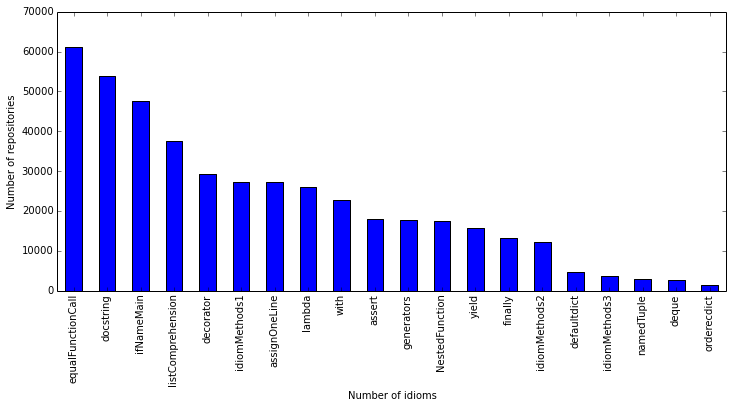
\includegraphics[width=80mm]{img/num_idiom_repo.png}
\label{fig:idiom_ranking}
\caption{Pythonic idioms ranking}
\end{figure}

Others of the most used idioms, but are grouped in order of complexity, are the magic methods (methods that are invoked when you use certain syntax). In figure 2 we can see the number of occurrences of each of them without been grouped. 

\begin{figure}[ht]
\centering
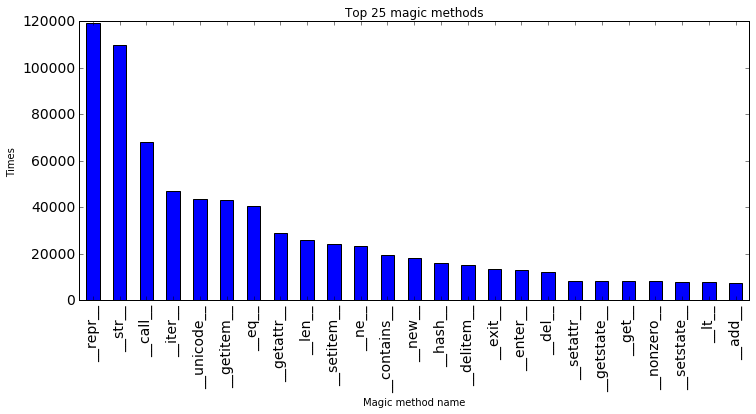
\includegraphics[width=80mm]{img/magic_methods.png}
\label{fig:magic_ranking}
\caption{Magic methods most common}
\end{figure}

One of the most usual is \verb|__init__|, but is omitted due to is necessary for creating a class and couldn't be consider a Python idiom.

The last figure shows the number of idioms in each repository. This curve show that many of the repository have few idioms, but actually more than 50\% have more than 40 idioms and the mean is 304.52.

\begin{figure}[ht]
\centering  
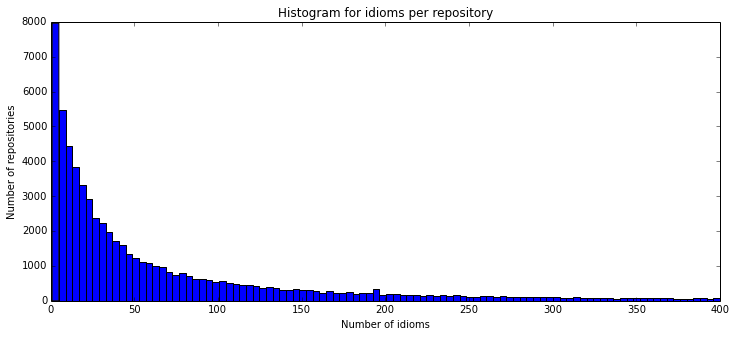
\includegraphics[width=80mm]{img/idioms_per_repository.png}
\label{fig:idioms_per_repository}
\caption{Number of idioms per repository}
\end{figure}


\section{Future work}

\bibliographystyle{abbrv}
\bibliography{references}


\end{document}

